\documentclass[conference]{IEEEtran}
\usepackage{blindtext, graphicx}
\usepackage[english]{babel}
\usepackage[utf8]{inputenc}
\usepackage{subfig}
\usepackage{xcolor,colortbl}
\usepackage{newtxmath}
\usepackage{spverbatim}
\usepackage{icomma}
\usepackage[subsection]{placeins}
\usepackage{lipsum}
\usepackage{listings}
\usepackage{color}
\usepackage{textcomp}
\definecolor{listinggray}{gray}{0.9}
\definecolor{lbcolor}{rgb}{0.9,0.9,0.9}
\lstset{
  backgroundcolor=\color{lbcolor},
  tabsize=4,
  rulecolor=,
  language=matlab,
  basicstyle=\scriptsize,
  upquote=true,
  aboveskip={1.5\baselineskip},
  columns=fixed,
  showstringspaces=false,
  extendedchars=true,
  breaklines=true,
  prebreak = \raisebox{0ex}[0ex][0ex]{\ensuremath{\hookleftarrow}},
  frame=single,
  showtabs=false,
  showspaces=false,
  showstringspaces=false,
  identifierstyle=\ttfamily,
  keywordstyle=\color[rgb]{0,0,1},
  commentstyle=\color[rgb]{0.133,0.545,0.133},
  stringstyle=\color[rgb]{0.627,0.126,0.941},
}
\usepackage{amsmath}

\captionsetup{belowskip=12pt,aboveskip=4pt}

\hyphenation{op-tical net-works semi-conduc-tor reglerteknik}


\begin{document}


\begin{titlepage}
  \begin{center}
    \vspace*{1cm}

    \Huge
    \textbf{Title}

    \vspace{0.5cm}
    \LARGE
    Subtitle

    \vspace{1.5cm}
    \Large
    \begin{tabular}[t]{c@{\extracolsep{8em}}c}
      Name 1 & Name 2\\
      email 1 & email 2 \\
      other 1 & other 2
    \end{tabular}
    \vfill

    \vspace{0.8cm}
    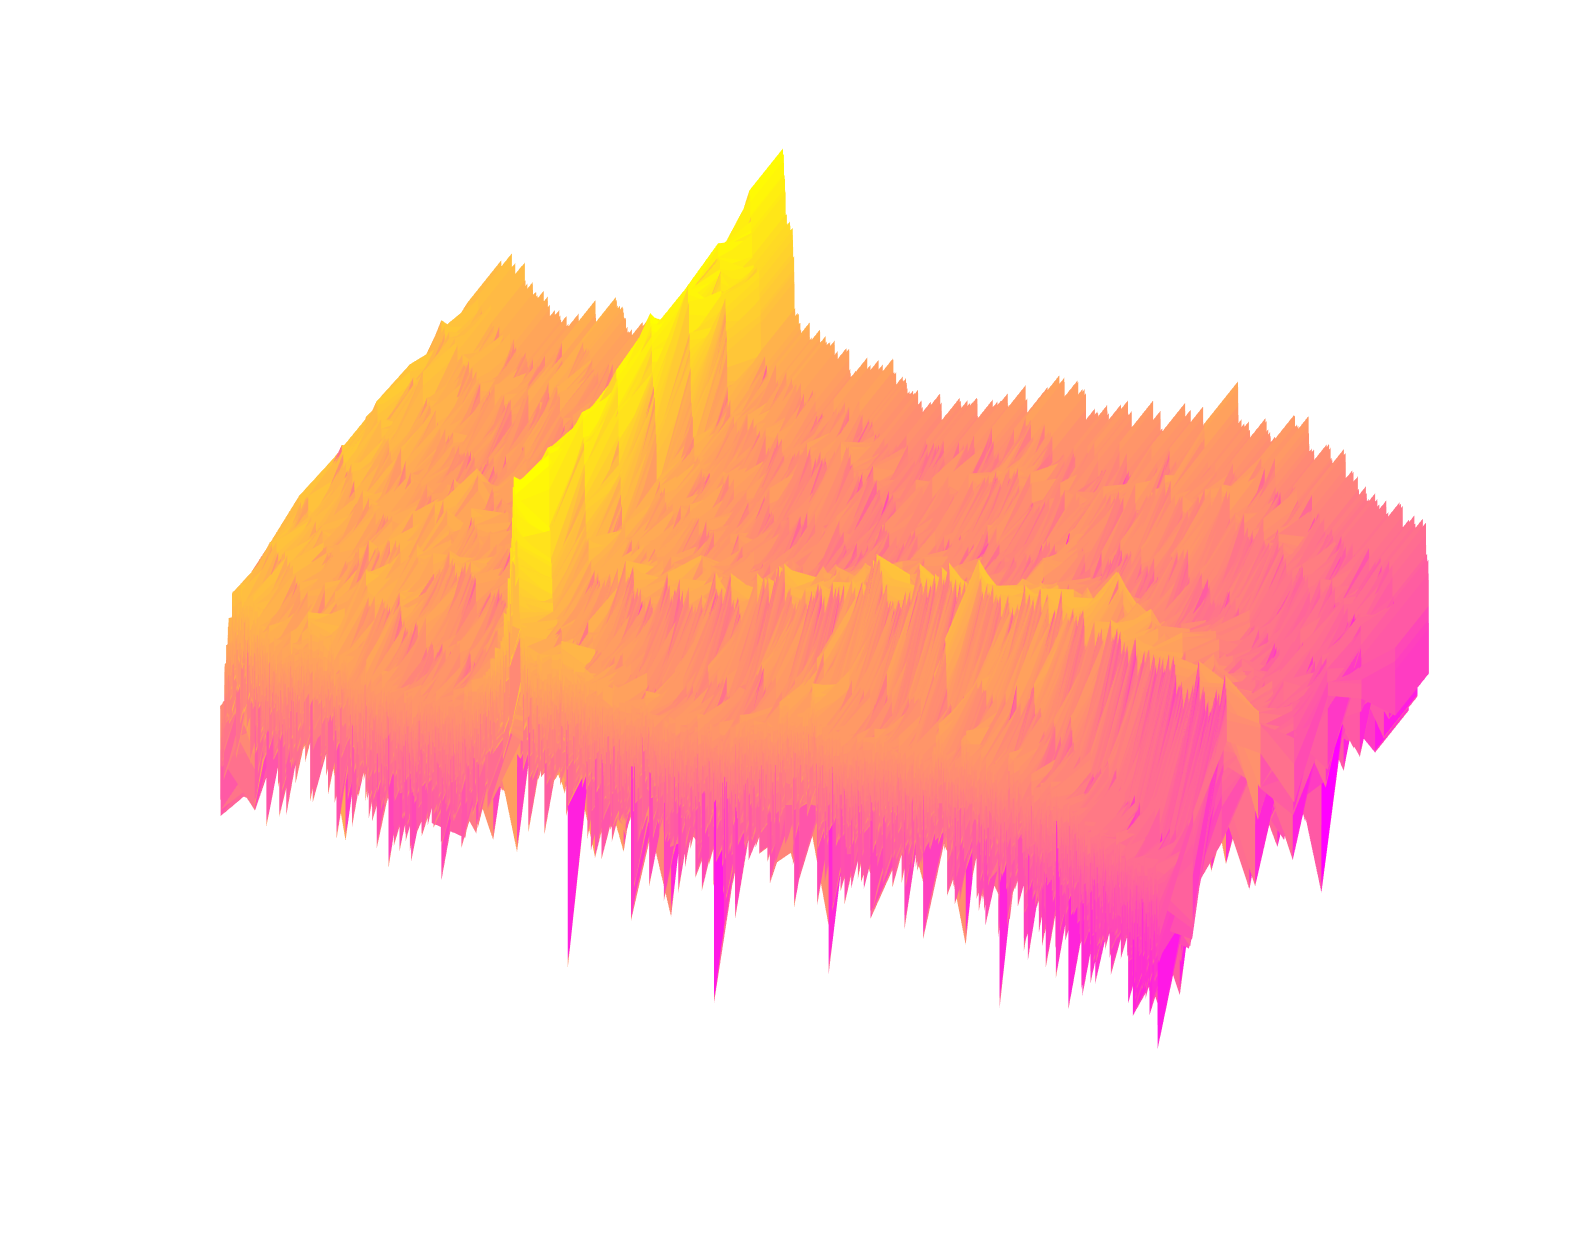
\includegraphics[width=\textwidth]{images/frontpage.eps}

  \end{center}
\end{titlepage}

\onecolumn
\tableofcontents{}
\twocolumn
\pagestyle{plain}

\section{Introduction}
\blanktext

\section{Theoretical Background}
\blanktext
\subsection{subsection}
\blanktext

\section{Section 2}

\subsection{Implementation}
\lstinputlisting{code/example.m}

\subsection{Results}

\begin{figure}
  \centering
  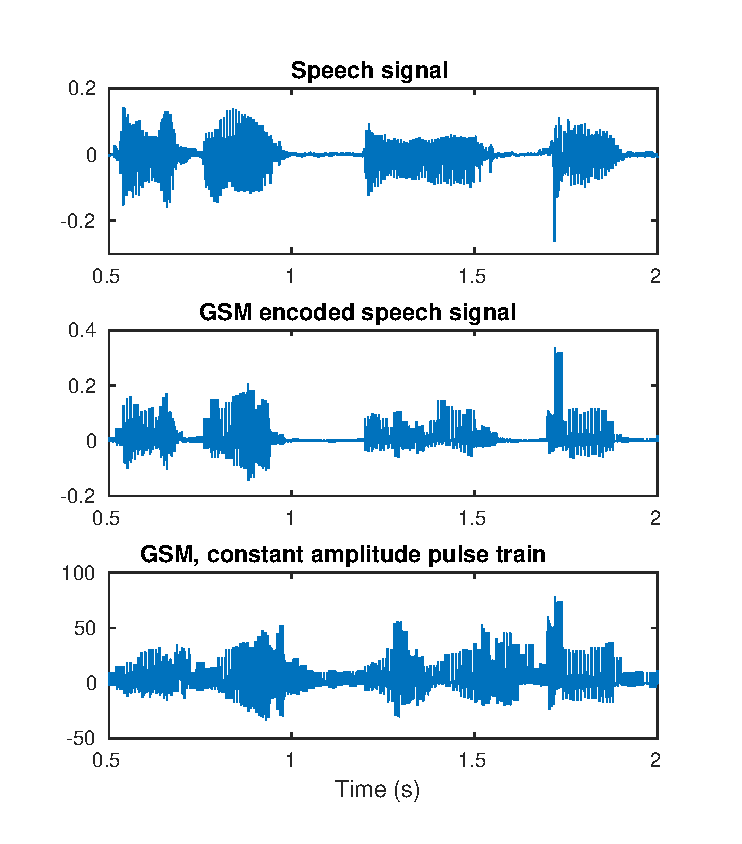
\includegraphics[width=\linewidth]{images/example.eps}
  \caption{Foobar}
  \label{fig:fig-label-1}
\end{figure}


\begin{thebibliography}{1}

\bibitem{kompendium}
  M. Enqvist et al. \emph{Industriell reglerteknik. Kurskompendium}
  Reglerteknik, Institutionen för systemteknik, Linköping University.

\bibitem{pm}
  \emph{Modellbaserad prediktionsreglering av destillationskolonn. Laborations-PM}
  Reglerteknik, Institutionen för systemteknik, Linköping University.

\end{thebibliography}

\clearpage

\onecolumn
\appendix
\lstinputlisting{code/example.m}

% that's all folks
\end{document}
